\section{Flow of images to splits}\label{app:folds-splits-viz}
The splits are created as described in \cref{subsubsec:slicom-folds}.
The process is visualized in \cref{fig:folds-splits-viz}.

\begin{figure*}
    \centering
    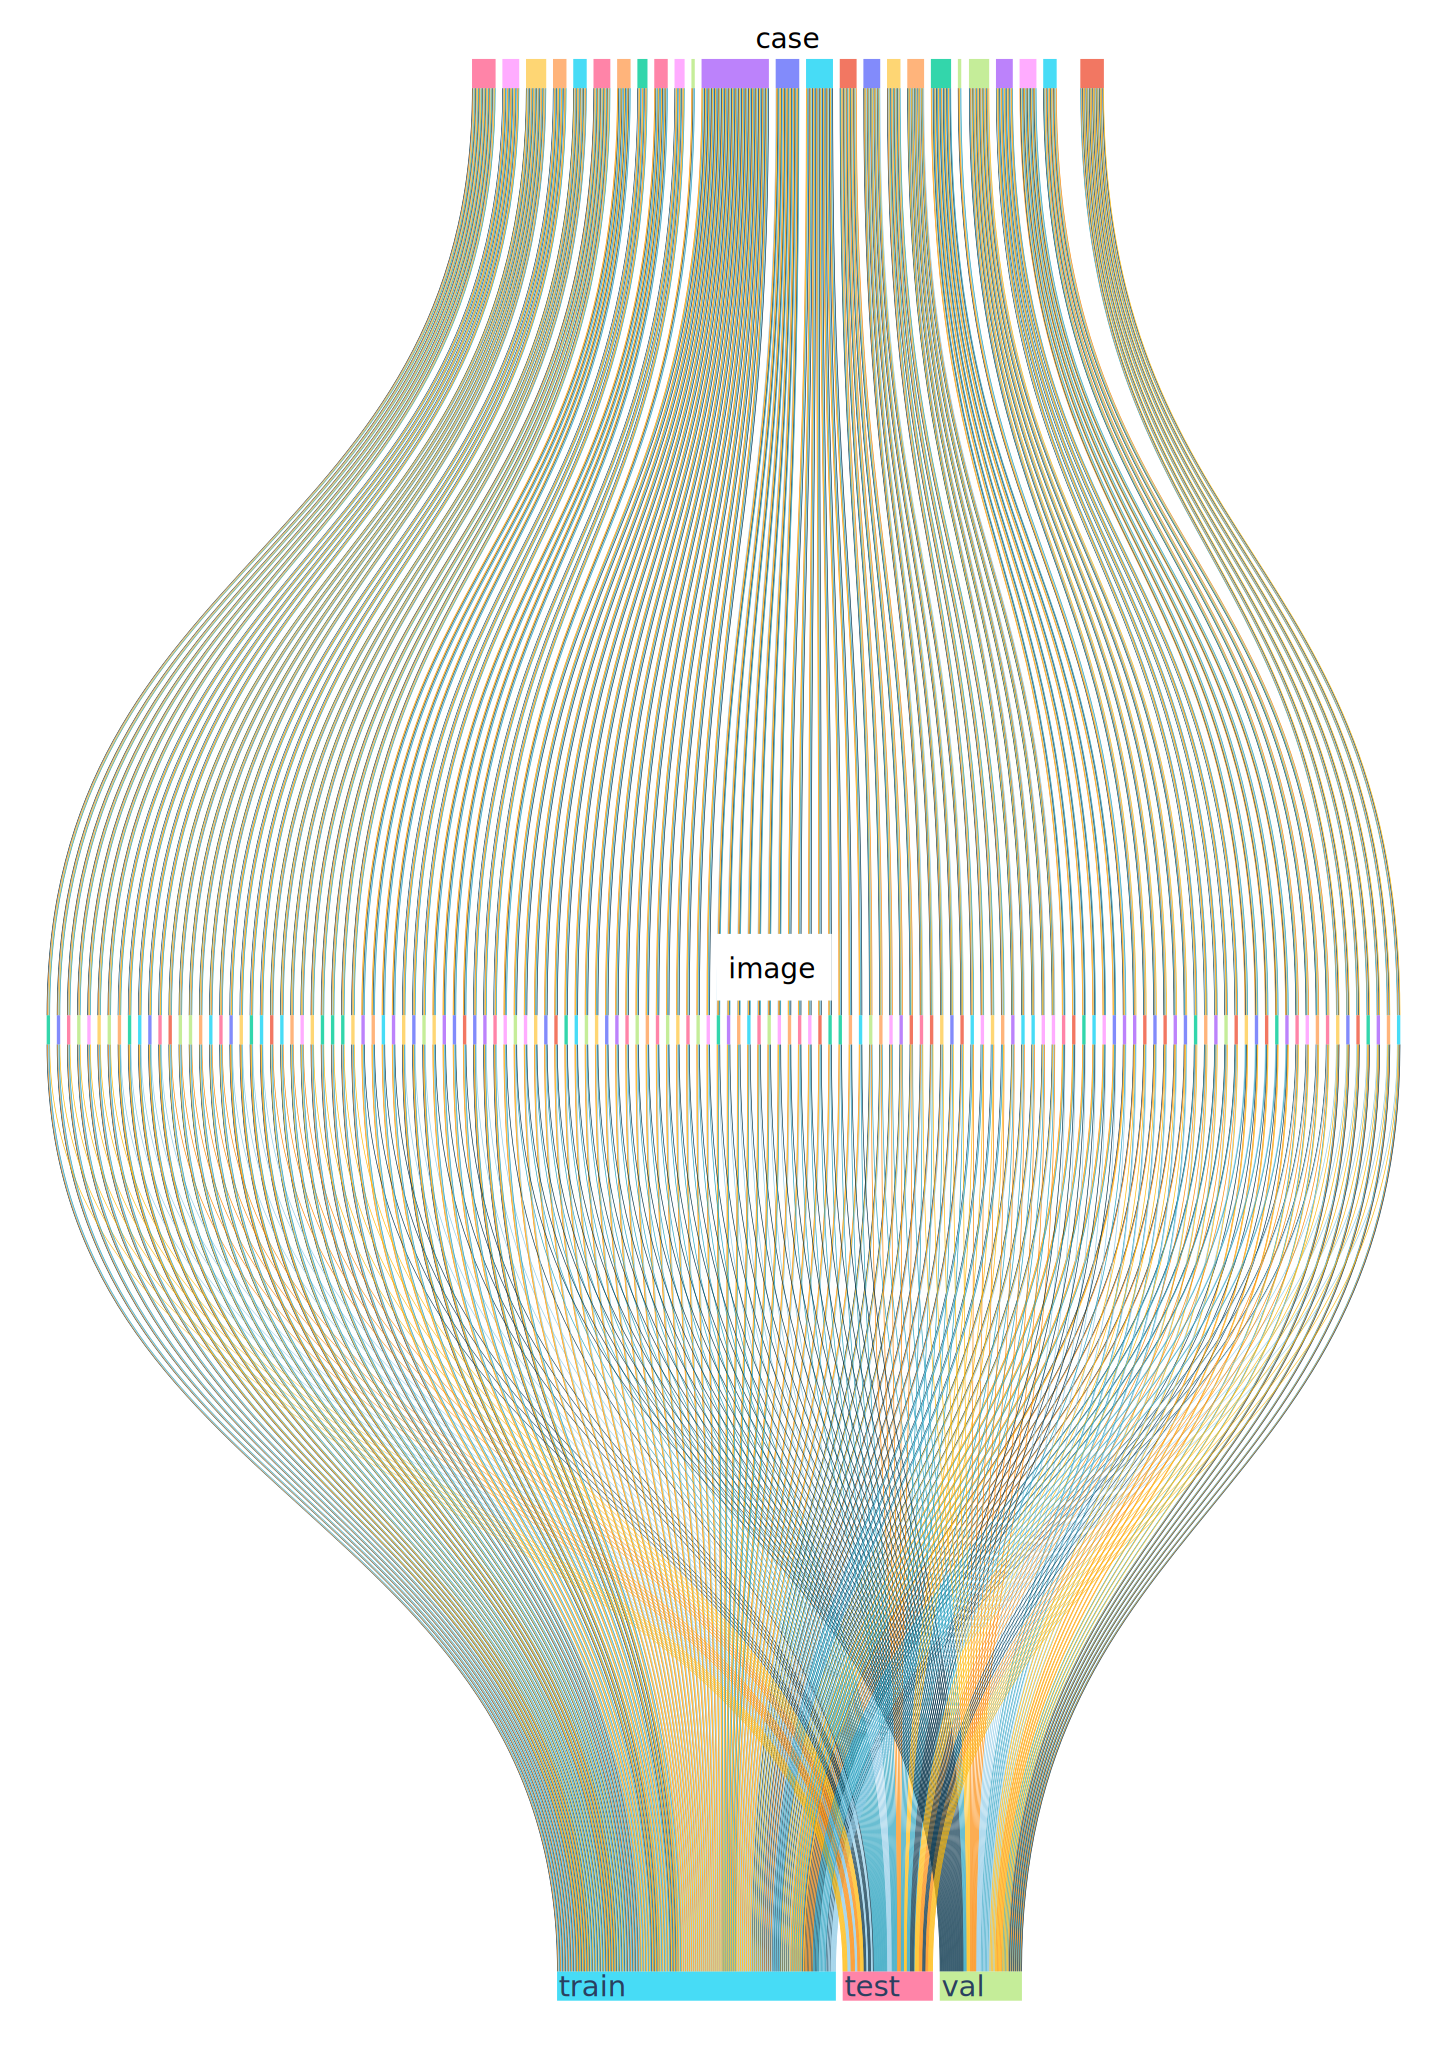
\includegraphics[height=0.55\paperheight]{pediatric-brain-tumours/images/folds-splits-viz.pdf}
    \caption[Flow of images to splits]{
        The flow of images to splits.
        Top row shows available cases.
        Every block is one case.
        Middle row shows available images and is linked to the cases.
        Bottom row shows training, validation and test splits.
        Colors show flow within one fold.
    }
    \label{fig:folds-splits-viz}
\end{figure*}
